\section{Definitions}
\label{sec:partialtree}

In this section, we introduce our novel tree structure, partial tree. Parital
tree  is used to process XPath queries over an XML documents in parallel. To use
partial tree, we first split an XML document into many chunks and then from
these chunks, we can construct multiple partial trees from the chunks. To deeply
understand what partial tree is, we first give some definitions for it.


To begin with, we give the defintion of types of element nodes. A partial
tree contains four different types of element nodes as shown in
Figure~\ref{fig:nodetypes}. The four types of element nodes in the figure are:
\emph{close node},  \emph{left-open node},  \emph{right-open node} and
\emph{pre-node}. A closed node is a regular node that has both its start tag and
end tag. For a node that does not have both of its tags, we call it \emph{open
node}, including left-open node, right-open node and pre-open node. A left-open
node has only its start tag, while a right-open node has only its end tag. In
case a node loses both of its tags, we call it \emph{pre-node}.

Open nodes are not a new concept. Kakehi et al~\cite{KaME07} proposed a new
approach for parallel reductions on trees and explicitly used 'open' nodes in
their paper. Choi et al.~\cite{ChLL14} proposed an idea to label nodes in split
chunks of a large XML documnet. Although they did not use the term, but the idea
is exact the same as that of open nodes.

A pre-open node is a novel idea proposed in our study and is different from the
other two open nodes that it comes from no tag, i.e. we do not create a pre-node
directly from the corresponding tags. This is becuase the corresponding tags of
a pre-node do not exist in the chunk.  This is, on the contrary, the most
significant idea of this study, so that we can use it to represent the missing
nodes on the path from the root of the whole tree to current subtrees parsed
from a chunk, which specifies the relationships between the root of the whole
tree and the substrees.

Note that (1) since our research focuses on evaluating queries on partial trees,
more specifically, mainly on element nodes, in case no tag is contained in a
chunk, we merge it to the next chunk until there is at least a tag existed in
the chunk (this is very rare case only when a context is too large or the chunk
is too small); (2) all open nodes, including pre-node, are element nodes.
Therefore, we omit attribute and content nodes in this section for
simplicity.

% Attribute and context nodes have been introduced in Chapter 3.


For representing open nodes separately from the close nodes in figures, we add
one black dot: $\bullet$ to an open node representing the side on which the node
is open, i.e. which tag is missing. For the example, when we split the pair of
tags \texttt{<A></A>} into two tags, we can create an right-open node A$\bullet$
from \texttt{<A>} and a left-open node $\bullet$A from \texttt{</A>}.


Last, based on the above definitions, we now give the definition to partial
tree. A partial tree is a tree structure with open nodes and represents a chunk
of an XML document and can be used for parallel XML processing.


\begin{figure}[t]
\centering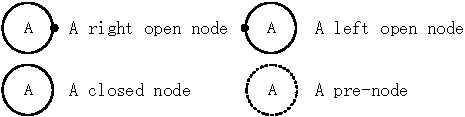
\includegraphics{partialtree/figures/fromWord-2.pdf}
\caption{Four types of element nodes}
\label{fig:nodetypes}
\end{figure}
